\documentclass{article}
\usepackage{spconf,amsmath,graphicx}

\input{../definitions.tex}


\title{Ranking of Gene Regulators through Differential Equations and Gaussian Processes}

\name{Antti Honkela$^1$, Matthew Holley$^2$, Marta Milo$^2$, Magnus
  Rattray$^3$, and Neil D. Lawrence$^3$\thanks{A.H. was supported by
    Postdoctoral Researcher's Project No 121179 of the Academy of
    Finland.  M.R. and N.D.L acknowledge support from EPSRC Grant No
    EP/F005687/1 "Gaussian Processes for Systems Identification with
    Applications in Systems Biology".  This work was supported in part
    by the IST Programme of the European Community, under the PASCAL2
    Network of Excellence, IST-2007-216886. This publication only
    reflects the authors' views.}}
\address{$^1$ Department of Information and Computer
    Science,\\ Aalto University School of Science and Technology,
    Helsinki, Finland\\
  $^2$ Department of ???, University of Sheffield, UK \\
  $^3$ School of Computer Science, University of
    Manchester, UK}

\begin{document}

\maketitle

\begin{abstract}
\end{abstract}

\section{INTRODUCTION}

Gene regulation is at the heart of how cells operate. In transcription
genes  whoch are  encoded in  the  DNA are  transcritbed to  messenger
RNA.  The  quantity of  RNA  transcribed  can  be measured  genomewide
through the  well established approach of gene  expression arrays. The
mechanisms  by   which  transcription  is  controlled   are  of  great
importance for medicine and biology.  Expression of a gene is switched
on  and off through  transcription factors  (TFs). These  are proteins
which bind to the DNA. The  TF proteins are produced by translation of
mRNA  to  protein.  The  mRNA  of the  transcription  factor  is  also
transcribed from  the genome.  This implies that  at the heart  of the
cell there is a network of TFs controlling the regulation of genes and
governing  the function  of  the  cell. Unpicking  this  network is  a
central  aim of  computational systems  biology. High  throughput gene
expression experiments allow the expression  level of many genes to be
assessed  simultaneously.  A typical  analysis  involves  a series  of
experiments  (perhaps a  time  series) for  which  gene expression  is
obtained.  Then   cluster  analysis  can   be  performed  and   it  is
hypothesized that genes that are  members of the same cluster (and are
therefore   probably  well   correlated   to  one   another)  may   be
coregulated.  Confirmation  experiments  may then  involve  ``knocking
out'' the  regulating gene and looking  for a resulting  change in the
gene expression of the hypothesized targets.

\subsection{Model Based Ranking}

Recently a  model based  approach to ranking  of targets  was proposed
that extends  this idea to  include an explicit  differential equation
model of  the gene expression \cite{Barenco:ranked06}. This  allows ranking of
coregulated genes  even when the expression profiles  are not strongly
correlated due to  low decay rates. The basic form of  the model is as
follows
\begin{equation}
  \diff{m_i(t)}{t} = b_i + s_i p(t) - d_i m_i(t)
\end{equation}
where the mRNA concentration of the $i$th gene, $m_i(t)$ is assumed to
be  regulated by  the TF  of interest,  $p(t)$, through  a sensitivity
parameter $s_i$.  The decay  rate of  the mRNA is  given by  $d_i$ and
$b_i$  is a  basal rate  of transcription.  Solution of  this equation
gives
\begin{equation}
  m_i(t) = a_i e^{-d_it} \frac{b_i}{d_i} + s_i
  e^{-d_it}\int_0^tp(u)e^{d_i u}\mathrm{d} u \label{eq:linearOperator}
\end{equation}
and the initial condition is given by $m_i(0)=a_i + \frac{b_i}{d_i}$. 

If coregulated targets have similar decay rates, they will be strongly
correlated, but  if decay  rates differ then  targets can  become more
weakly correlated.  The  idea behind a ``model based  approach'' is to
consider that  coregulated targets should conform  to the differential
equation. Thus  we see  a TF activity,  $p(t)$, that  explains targets
simultaneously through  a range of different decay  rates.  Clearly we
are also making further assumptions  here: for example we are assuming
TFs  don't act  in tandem  and  that the  response to  the TF  doesn't
saturate. However,  the model is  richer than the  standard genomewide
analysis   techniques  of  seeking   correlation  or   clustering  the
data. This model based approach to gene regulation was also considered
by  \cite{Gao:latent08}. They  used Gaussian  process priors  over the
unobserved TF activity  to create a fully probabilistic  model for the
coregulated genes.  Likelihoods can then  be used to rank these models
and determined which genes are likely to be coregulated.

Also in \cite{Gao:latent08} this framework was extend by introducing a
simple model  of translation.  Let's represent the  mRNA governing the
transcription factor by $m_0(t)$. Let's assume that this is translated
to  $p(t)$ through a  process that  can be  modelled by  the following
differential equation
\begin{equation}
  \diff{p(t)}{t} = \sigma m_0(t) - \delta p(t).
\end{equation}
Once again this  is a significant simplification. It  assumes that the
TF  protein is  produced from  only one  mRNA and  ignores potentially
important post translational  modifications such as phosphorylation or
ubiquitination (spelling!).

Given  observations  from the  potential  target  mRNA, $m_i(t)$,  and
observations  from the  governing TFs  mRNA a  joint  Gaussian process
likelihood can be constructed  and maximized with respect to $\delta$,
$\sigma$,  $a_i$,  $b_i$,  $s_i$  and  $d_i$.  For  a  given  TF  this
likelihood can be measured for all potential target genes and they can
then  be  ranked as  putative  targets.  This  idea was  exploited  by
\cite{Honkela:modelbased10} who  validated their results using ChIP
data and were
able to  show that model  based approaches can do  considerably better
than simple correlation based approaches.

In this  paper we want to turn  this idea on its  head. An alternative
question a biologist may ask is  given a particular gene, what are the
likely regulators  of that gene. In  other words we  are interested in
ranked regulator prediction instead  of ranked target prediction. This
problem will generally  be harder than target prediction  as there are
likely  to  be  many  targets   of  a  particular  TF,  but  only  few
regulators.  However, we  can  restrict ourselves  to  known TFs  when
searching for regulators and this  reduces the number of genes we have
to  search  through  from  thousands  to  hundreds.  Ranked  regulator
prediction (RRP)  has the potential  to provide biologists with  a new
tool for probing their regulatory networks.

In the remainder of this paper we will review the Gaussian process
approach to modelling transcriptional regulation and demonstrate our
ideas on a real world biological problem. Despite the simplifying
assumptions we make, we show very promising results.

\section{Gaussian Process Modelling}

A  Gaussian  process (GP)  is  a  probabilistic  prior over  functions
\cite{Rasmussen:book06}.  A GP  provides a  nonparametric  approach to
modelling data. The  basic idea is that observations  of a function of
interest,   $p(t)$,   given  by   $\mathbf{p}   =  \left[p_1,   \dots,
  p_T\right]^\top$,   where    $p_i=p(t_i)$   are   jointly   Gaussian
distributed,
\begin{equation}
  \mathbf{p} \sim \mathcal{N}(\mathbf{0}, \mathbf{K}).
\end{equation}
where the elements of the  covariance matrix are given by a covariance
function. This may  be any function that leads  to a positive definite
matrix, but a common choice is the Gaussian covariance,
\begin{equation}
  k(t_i,   t_j)   =  \frac{1}{\sqrt{2\pi   \ell^2}}\exp\left(-\frac{(t_i
      -t_j)^2}{2\ell^2}\right).
\end{equation}
Whilst we usually  think of Gaussian's as being  densities over finite
length vectors, the process perspective  allows us to think of them as
distributions over infinite length vectors. The important idea is that
the  other  possible things  that  could  be  happening are  all  been
marginalized, and we only  deal with the observations $\mathbf{p}$. If
we need to  query a new observation time, $p_*$,  we express the joint
distribution over the augmented variable set as
\begin{equation}
  \left[\begin{matrix}
      \mathbf{p}\\
      \mathbf{p}_*
    \end{matrix}\right]
  \sim \mathcal{N}\left(\mathbf{0}, \left[\begin{matrix}
        \mathbf{K} & \mathbf{K}_{:,*}\\
        \mathbf{K}_{*,:} & \mathbf{K}_{*,*}
      \end{matrix}
    \right]\right),
\end{equation}
where $\mathbf{K}_{:,*}$  is the covariance  function computed between
the training  times, $\mathbf{t}$, and the  test times, $\mathbf{t}_*$
and $\mathbf{K}_{*,*}$ is the covariance function computed between the
test times.

Simple  manipulation of  this joint  Gaussian  density, $p(\mathbf{p},
\mathbf{p_*}|\mathbf{t},  \mathbf{t}_*)$,  allows  us to  compute  the
conditional density of the test data given the training data,
\begin{equation}
  p(\mathbf{p}_* | \mathbf{p}, \mathbf{t}, \mathbf{t}_*) = \mathcal{N}\left(\mathbf{p}_*|\boldsymbol{\mu}, \boldsymbol{\Sigma}\right)
\end{equation}
where
\begin{equation}
  \boldsymbol{\mu} = \mathbf{K}_{*,:}\mathbf{K}^{-1}\mathbf{p}
\end{equation}
and 
\begin{equation}
  \boldsymbol{\Sigma} = \mathbf{K}_{*,*} - \mathbf{K}_{*,:}\mathbf{K}^{-1}\mathbf{K}_{:,*}.
\end{equation}

The simple translation/transcription model we described in the last
section gives a deterministic relationship between the TF activity,
$p(t)$ and the gene expression levels, $m_0(t)$ and $m_i(t)$. This
deterministic relationship can be encoded within a Gaussian process by
noting that it is given by a \emph{linear operator}. The linear
operator in question is the convolution of the function with an
exponential (see \refeq{eq:linearOperator}). A convolution of a
Gaussian process with a deterministic function leads to another
Gaussian process: this results from two properties, a Gaussian process
multiplied by a deterministic function is also a Gaussian process and
the integral of a Gaussian process is also a Gaussian process. The
other effect of \refeq{eq:linearOperator} is to introduce a new mean
function through the addition of $\frac{b_i}{d_i}$ and $a_i e^{-d_i
  t}$. Details are given in
\cite{Lawrence:transcriptionalGP06,Gao:latent08,Honkela:modelbased10}
but the
main result is that the cross covariances between the TF concentration
and the mRNA concentrations can be computed:
\begin{equation}
  .
\end{equation}
where $k_{p,i}(t, t^\prime)$ gives the covariance between the TF
concentration and the mRNA associated with the $i$th gene at times $t$
and $t^\prime$. This suggests a model for the gene expression which is
jointly Gaussian and has the form
\begin{equation}
  .
\end{equation}

\section{Experiments}

We tested the method by looking for candidate regulators of Gata3 gene
in mouse.  Gata3 is itself a transcription factor with many important
functions~\cite{Chou2010}.  It is, for example, critical in the
development of hair cells in the inner ear.  Mice and humans with just
one of the usual two copies of the Gata3 gene disabled are
deaf~\cite{Esch2000}.  Because of its many roles, Gata3 regulation is
very complex and its details are relatively poorly
understood~\cite{Burch2005}.

The expression data consisted of two time series from a cell line
model of mouse inner ear development~\cite{Helyer2007}.  Both time series
consisted of 6 time points, sampled at 0, 1, 2, 4, 7, and 14 days
after the cells are moved to a temperature that stimulates their
development.  In one of the time series the cells are untreated while
in the other they are exposed to retinoic acid, which focuses the
differentiation toward one of several possible cell types.  The
retinoic acid treatment does not affect the expression of Gata3 so we
used these two time series as if they were two repeated experiments.
This should automatically suppress genes with significant differential
expression under the two different conditions.  The expression data
was processed using the mmgMOS algorithm from the \emph{puma} R
package~\cite{Liu:tractable04,Pearson:puma09} from Bioconductor.  The
inferred posterior expression levels from mmgMOS were utilised to
obtain individual noise variances for each observation as described
in~\cite{Honkela:modelbased10} using the \emph{tiger} Bioconductor
package~\cite{Honkela:tigerpackage10}.

We first extracted a set of mouse TFs and probable TFs from the TFCat
database~\cite{Fulton2009}.  This yielded a list of 511 genes.  Out of
these, 365 were mappable on the array used in the expression
measurements.  These genes were represented by 493 independent probe
sets on the array.

Next, we fitted the GP models independently using each of these 493 TF
gene probes as the input and Gata3 as the output.  This was also
performed in R/Bioconductor using the \emph{tiger} package.  The genes
with the largest likelihood values are listed in
Table~\ref{tab:results}.

\begin{table}[htb]
  \centering
  \begin{tabular}{lll}
    Gene & log-likelihood & z-score \\
    \hline
    Prrx2 & -0.37 & 3.6 \\
    Tle3 & -0.47 & 4.5 \\
    Ctbp2 & -0.67 & 11.8 \\
    Esr2 & -1.37 & 1.1 \\
    Smarcd2 & -1.37 & 6.1 \\
    Six1 & -1.57 & 6.5 \\
    Runx2 & -2.16 & 3.9 \\
    Mtf2 & -2.56 & 6.2 \\
    Klf13 & -2.92 & 1.6 \\
    Six4 & -3.05 & 4.7 \\
  \end{tabular}
  \caption{Top-ranking genes in the experiment}
  \label{tab:results}
\end{table}

\begin{figure}[htb]
  \centering
  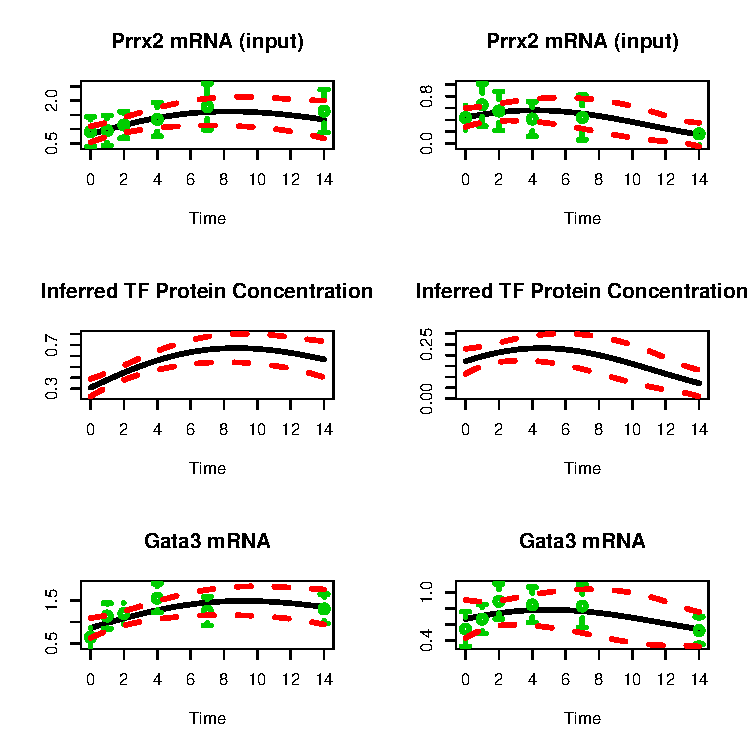
\includegraphics[width=\columnwidth]{gpdisim_Prrx2_Gata3}
  \caption{Top-ranking models}
  \label{fig:model1}
\end{figure}

\begin{figure}[htb]
  \centering
  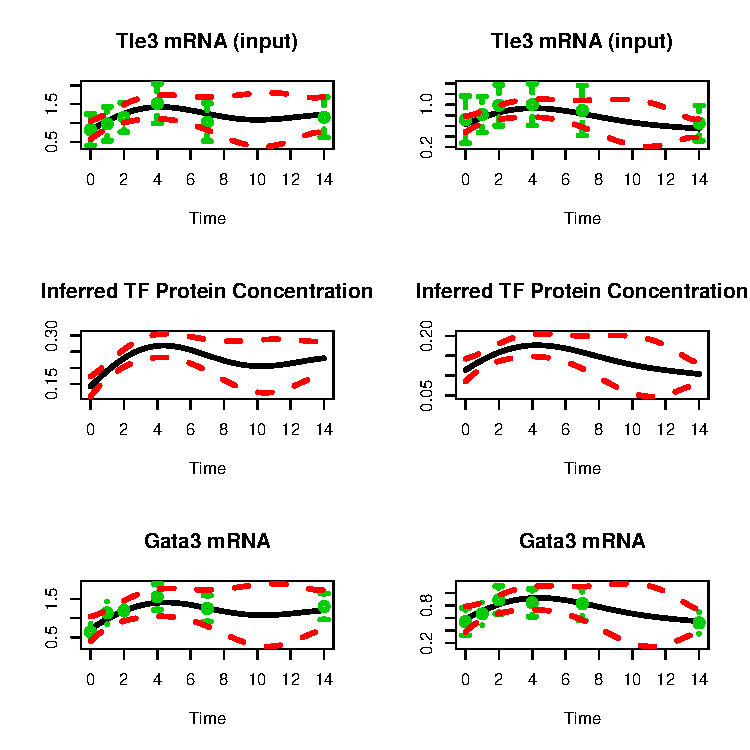
\includegraphics[width=\columnwidth]{gpdisim_Tle3_Gata3}
  \caption{Top-ranking models}
  \label{fig:model2}
\end{figure}

\begin{figure}[htb]
  \centering
  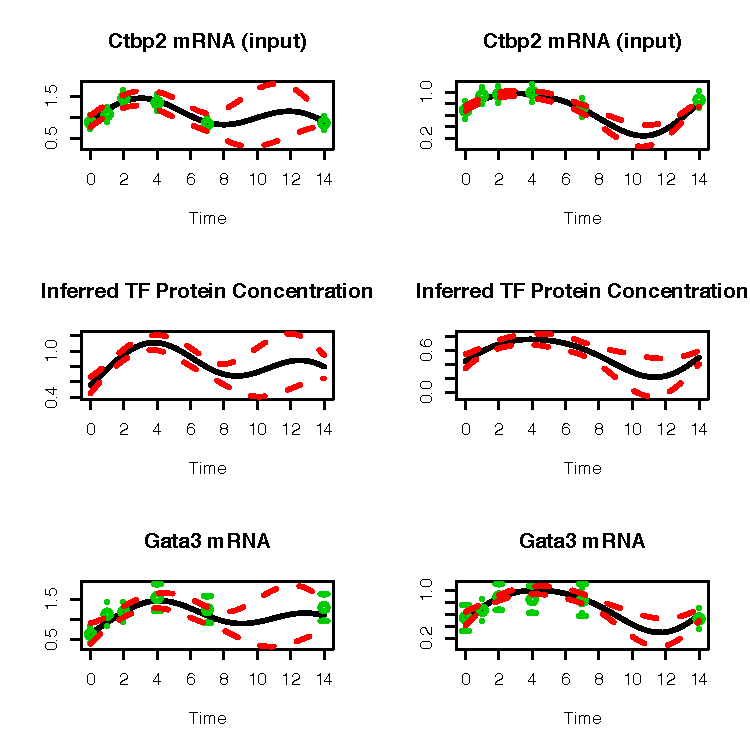
\includegraphics[width=\columnwidth]{gpdisim_Ctbp2_Gata3}
  \caption{Top-ranking models}
  \label{fig:model3}
\end{figure}

\begin{figure}[htb]
  \centering
  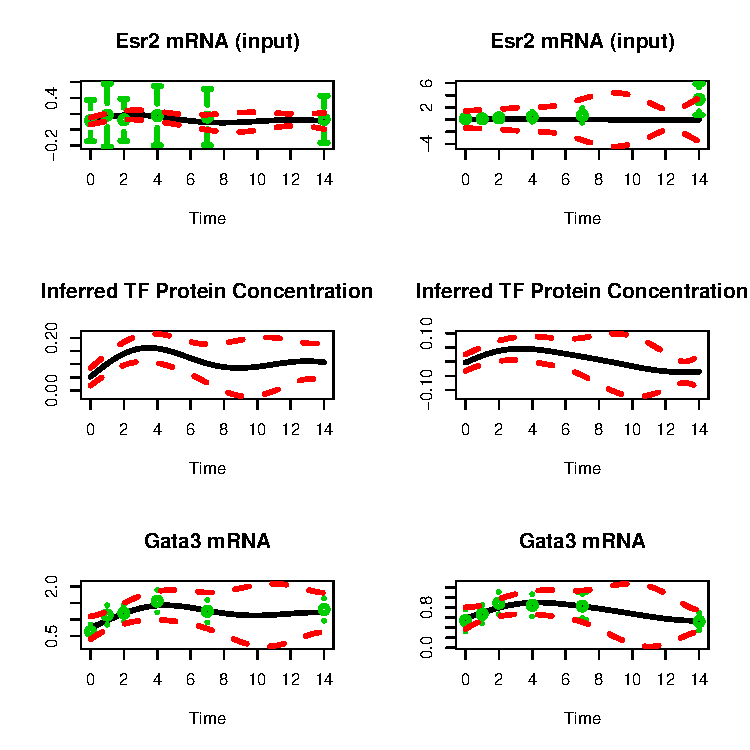
\includegraphics[width=\columnwidth]{gpdisim_Esr2_Gata3}
  \caption{Top-ranking models}
  \label{fig:model4}
\end{figure}

\begin{figure}[htb]
  \centering
  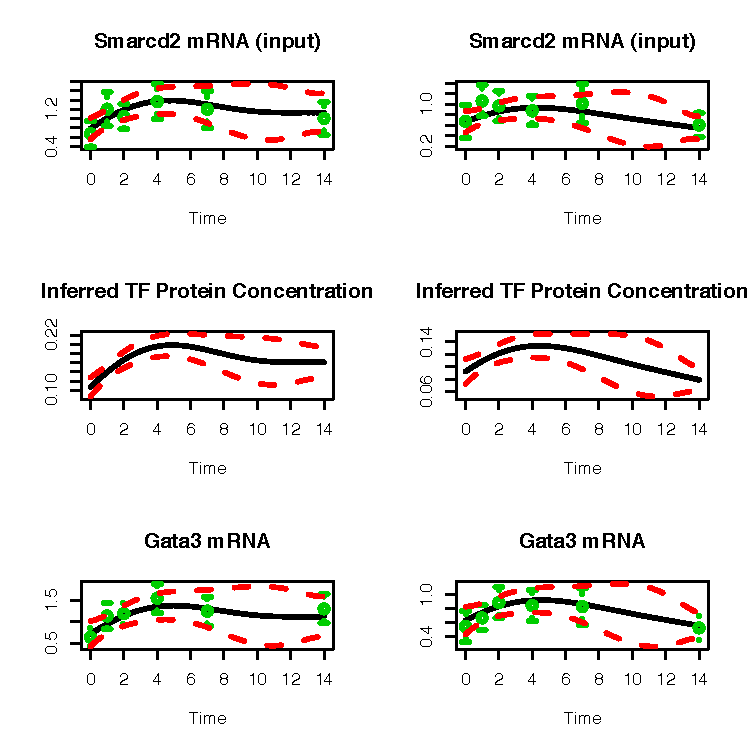
\includegraphics[width=\columnwidth]{gpdisim_Smarcd2_Gata3}
  \caption{Top-ranking models}
  \label{fig:model5}
\end{figure}

\section{Discussion}

\bibliographystyle{IEEEbib}
\bibliography{lawrence,other,zbooks}


\end{document}